% coding:utf-8

%----------------------------------------
%FOSADSVB, a LaTeX-Code for a summary of digital signal processing
%Copyright (C) 2015, Mario Felder & Michi Fallegger

%This program is free software; you can redistribute it and/or
%modify it under the terms of the GNU General Public License
%as published by the Free Software Foundation; either version 2
%of the License, or (at your option) any later version.

%This program is distributed in the hope that it will be useful,
%but WITHOUT ANY WARRANTY; without even the implied warranty of
%MERCHANTABILITY or FITNESS FOR A PARTICULAR PURPOSE.  See the
%GNU General Public License for more details.
%----------------------------------------
\chapter{Digitales Filterdesign}
Ziel: Bestimmen der Parameter $b_k$ \& $a_k$, sowie der Ordnung $N$ \& $M$ für gegebene Filterspezifikationen.
\begin{center}
	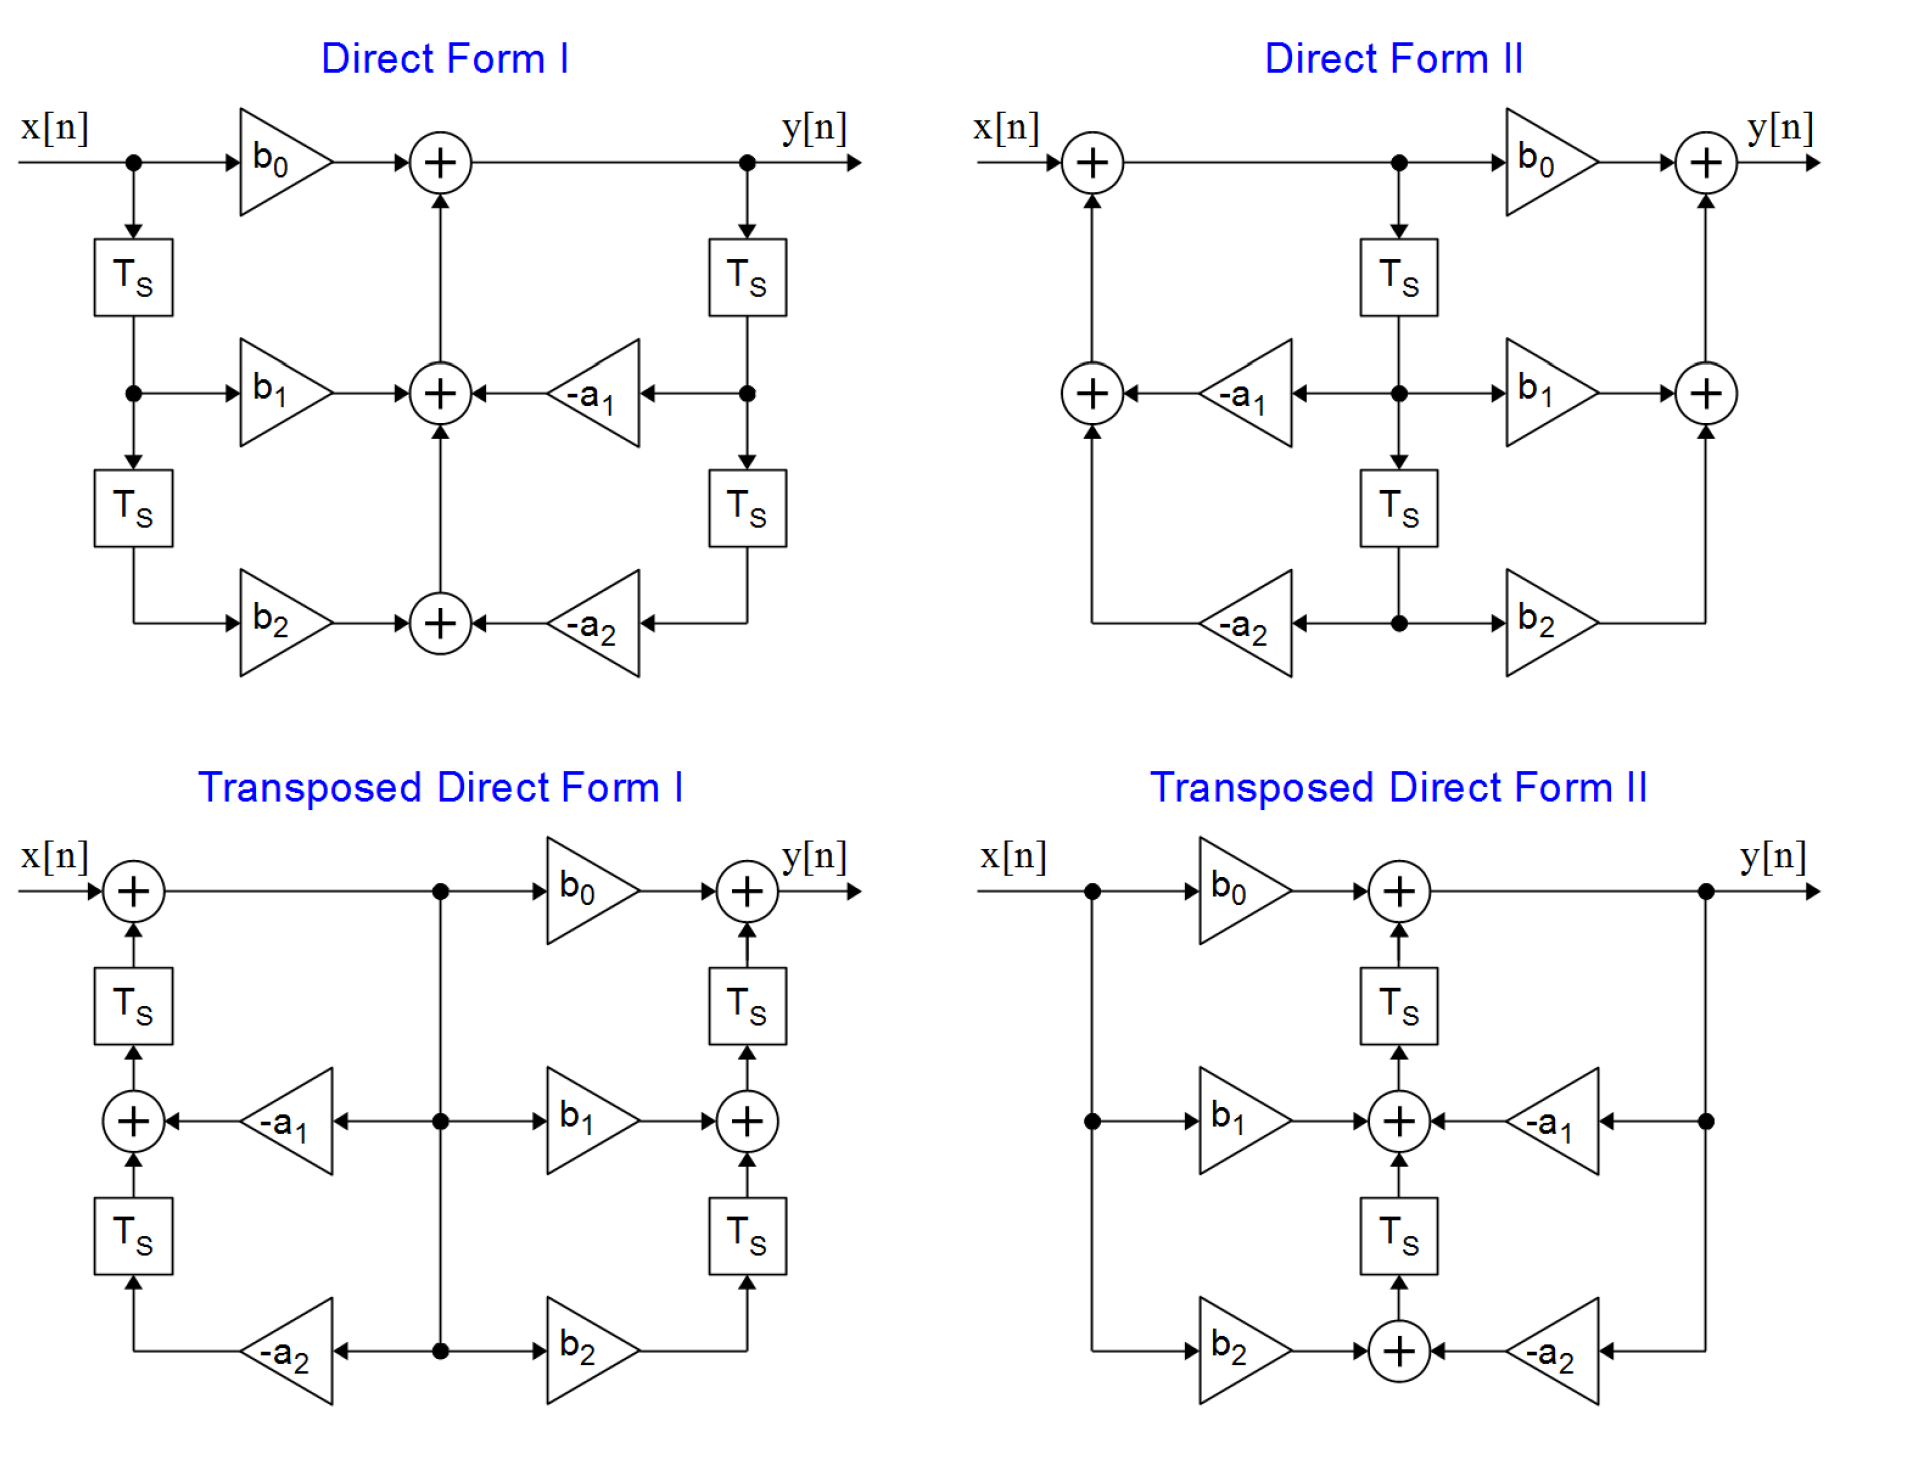
\includegraphics[width=.7\textwidth]{../fig/lti_scheme}
\end{center}

%===============================================================================
\section{Übertragungsfunktion}
Differenzengleichung:
\[y[n] = \sum_{k=0}^{N}b_k \cdot x[n-k]-\sum_{k=0}^{M} a_k \cdot y[n-k]\]
Übertragungsfunktion ($a_0$ normiert auf 1):
\[ H(z) = \frac{Y(z)}{X(z)} =
\frac{b_0+b_1 \cdot z^{-1} + b_2 \cdot z^{-2}+\ldots+b_N \cdot z^{-N}}
	{1+a_1 \cdot z^{-1} + a_2 \cdot z^{-2}+\ldots+a_M \cdot z^{-M}} \]
Amplituden, Phasengang:
\[ H(\Omega)=H(z)\big|_{z=e^{j\Omega}} \]
Beim Amplitudengang wird der Betrag $\big| H(\Omega)\big|$ in Abhängigkeit von $\Omega$ geplottet:\\
\[ \big| H(\Omega)\big| =  |K| \cdot \frac{|(z-z_1)||(z-z_2)|..|(z-z_N)|}
								{|(z-p_1)||(z-p_2)|..|(z-p_M)|}
								\cdot |z|^{M-N} \]
Phasengang: \[ \varphi(H(z)) = \sum_{k=1}^{N} \varphi(z-z_k) 
								-\sum_{k=1}^{M} \varphi(z-p_k)
								+\sum_{k=N+1}^{M} \varphi(z)  \]
Trick 1:
\[ 1-e^{-k \cdot jx} = e^{-\frac{k}{2} \cdot jx} \cdot (e^{\frac{k}{2} \cdot jx} - e^{-\frac{k}{2} \cdot jx})\]
Trick 2:
\[ sin(x)= \frac{e^{j \cdot x}-e^{-j \cdot x}}{2j} \hspace{20mm} 
cos(x)= \frac{e^{j \cdot x}+e^{-j \cdot x}}{2} \]
\textbf{Beispielaufgabe Phasenwinkel:\\} 
Analytisches Ermitteln des Phasenganges für die Übertragungsfunktion $H(z) = 1-z^{-4}$:
\begin{align*}
\angle H(\Omega)		 	&=\angle H(z)\big|_{z=e^{j\Omega}} \\
											&=\angle (1-e^{-4 \cdot j\Omega}) \\
\text{Anwenden von Trick 1:} 		&= \angle(e^{-2 \cdot j\Omega} \cdot (e^{2 \cdot j\Omega} - e^{-2 \cdot j\Omega})) \\
\text{Anwenden von Trick 2:} 		&= \angle(\underbrace{e^{-2 \cdot j\Omega}}_{= -2\Omega} 
\cdot \underbrace{2 \cdot j}_{+\frac{\pi}{2}} \cdot \underbrace{sin(2\Omega)}_{
\substack{ {0    \text{ für: } 0\leq \Omega \leq \frac{\pi}{2}} \\ 
           {+\pi \text{ für: } \frac{\pi}{2} \leq \Omega \leq \pi}}})
\end{align*}
Es gibt somit eine Fallunterscheidung für die zwei Bereiche von $\Omega$. Dies ist zuständig für den Phasensprung bei $\pi/2$. 
Graphische Darstellung des Phasenwinkels für das letzte Element (sinus):
\begin{center}
	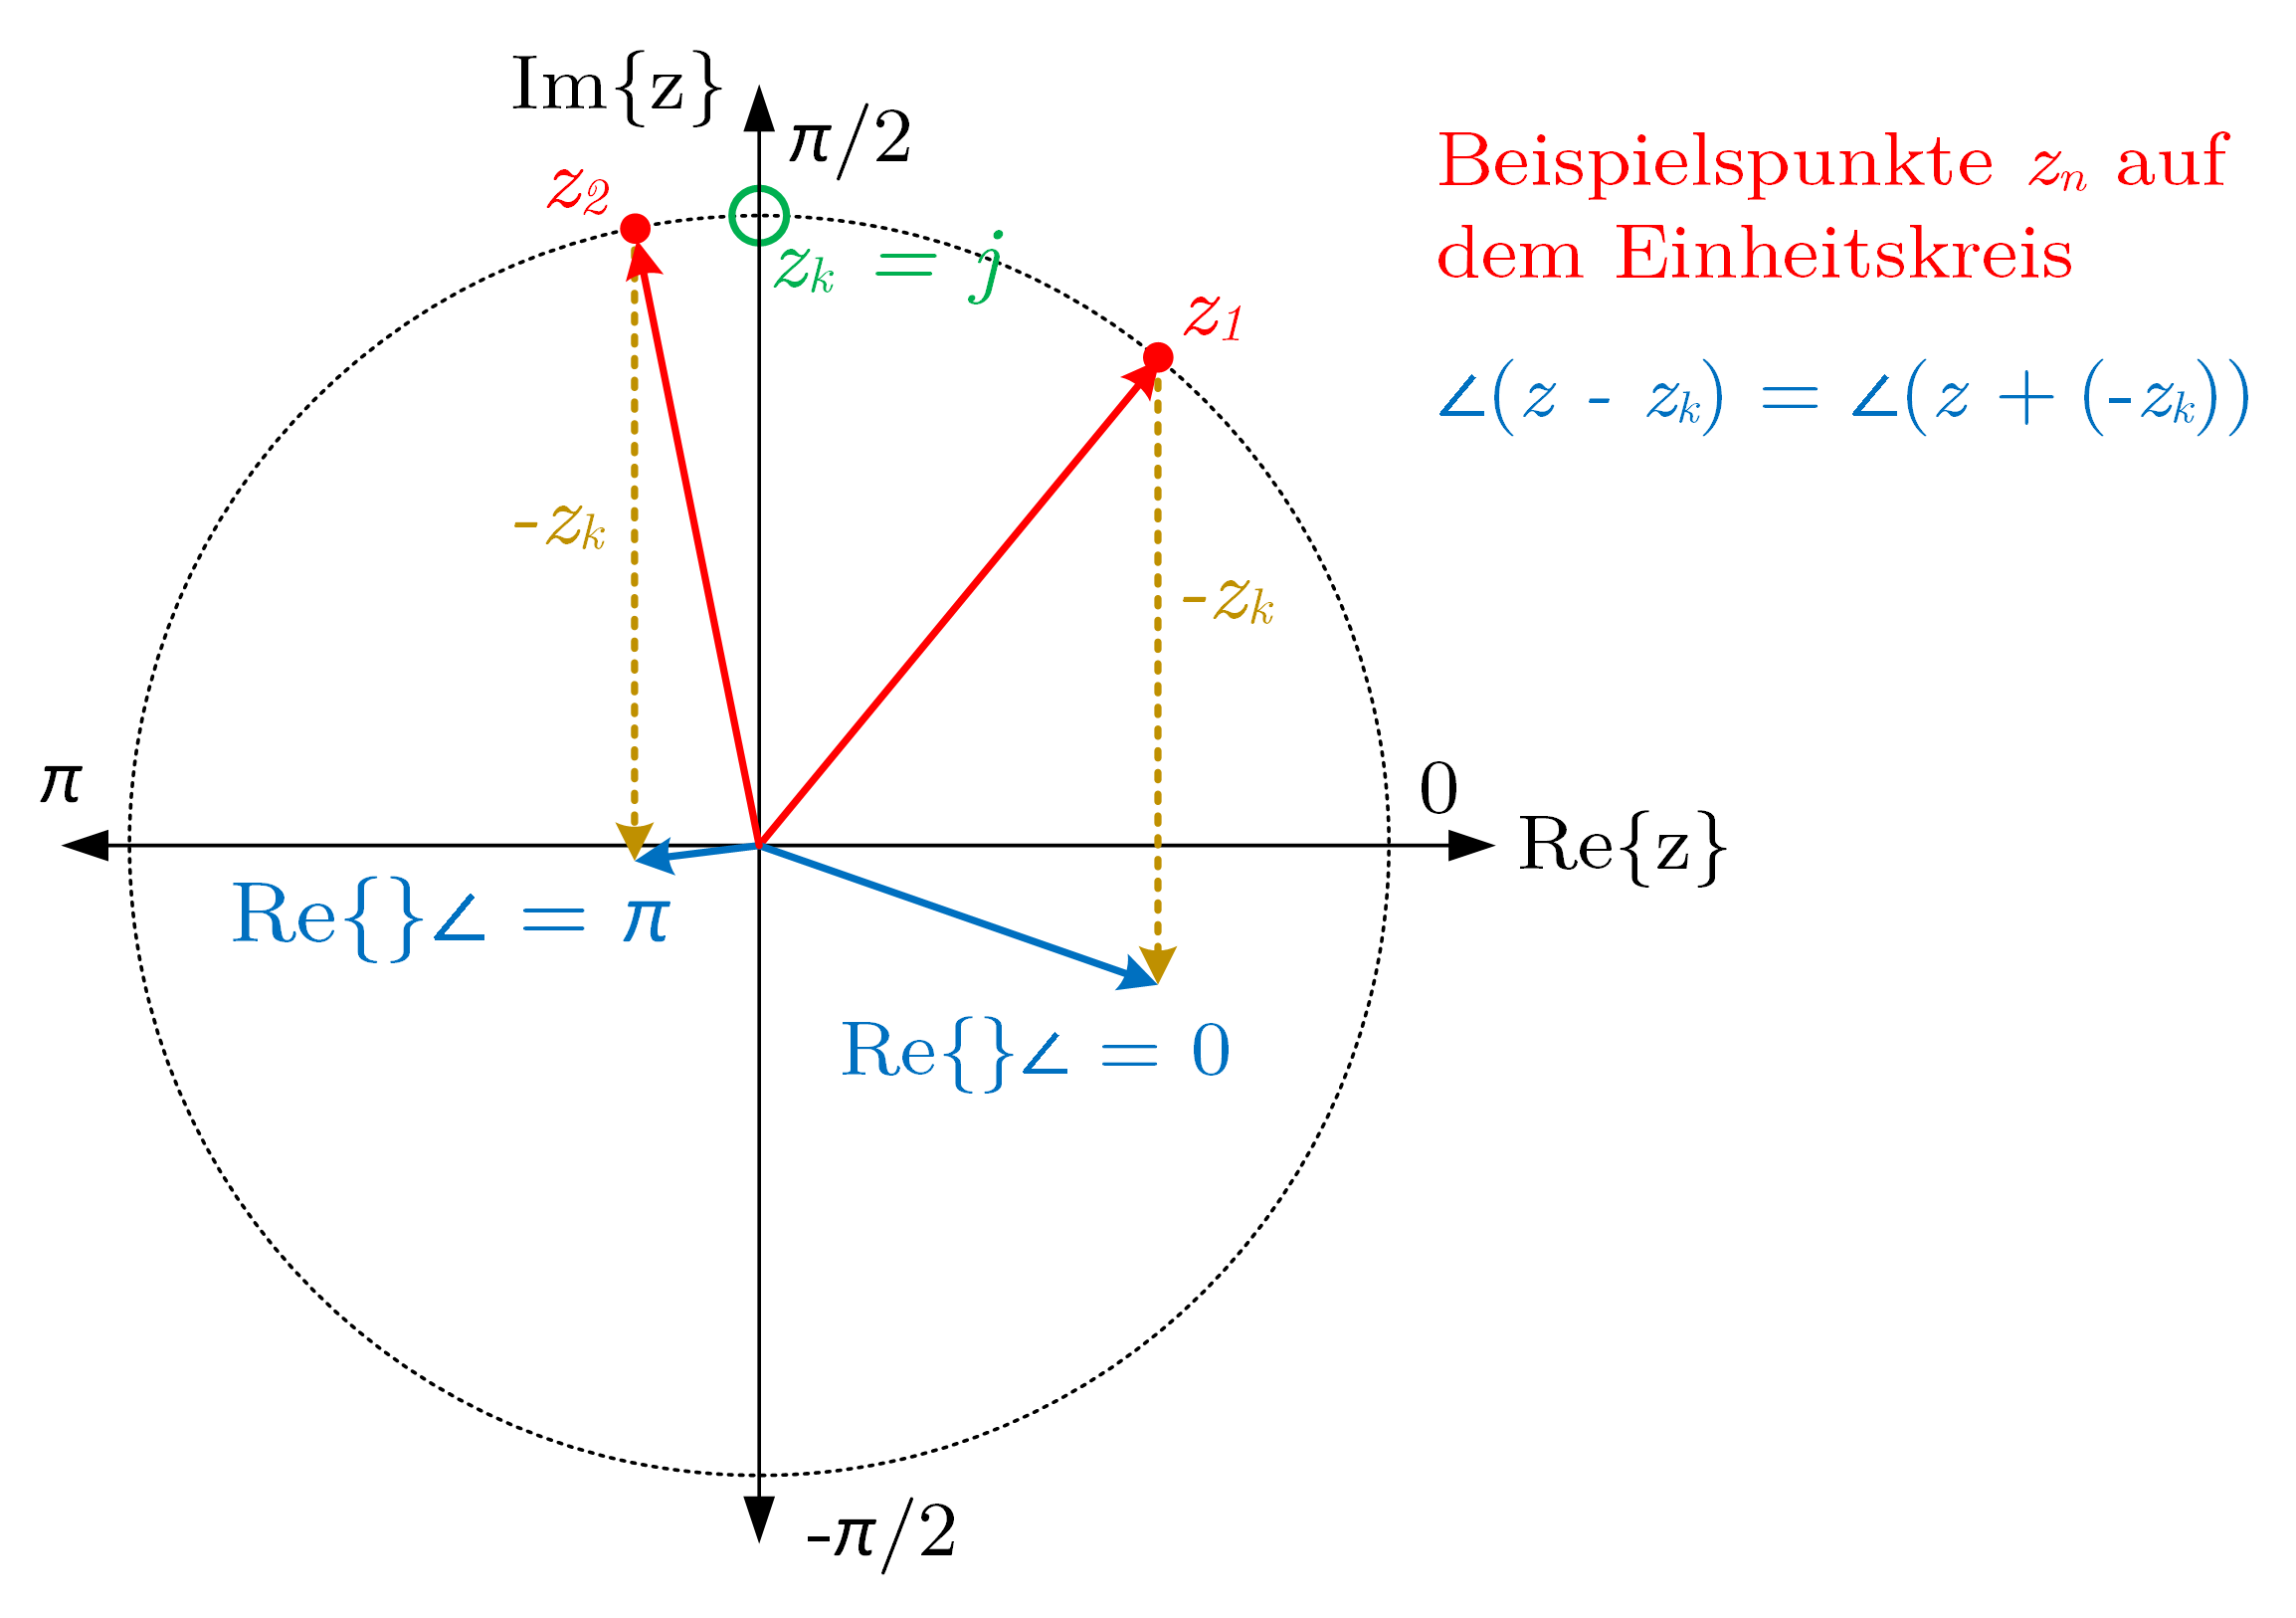
\includegraphics[width=.575\textwidth]{../fig/phasenwinkel_analyse}
\end{center}
\textbf{Beispielaufgabe Verstärkung:\\} 
Berechnen der Frequenz, bei der die Verstärkung $\big|H(z)\big|$ von $H(z) = 1-z^{-1} =\sqrt{2}$ ist:
\begin{align*}
 H(\Omega)	 	&= H(z)\big|_{z=e^{j\Omega}} \\
\big| H(\Omega)\big| &= \big|1-e^{-j\Omega}\big| = \frac{\big|e^{j\Omega}-1\big|}{\big|e^{j\Omega}\big|} 
          \Longrightarrow \big|e^{j\Omega}\big| \text{ aus dem Nenner} = 1 \\
\text{Verinfacht sich somit zu: }	\big| H(\Omega)\big| &= \big|e^{j\Omega}-1\big| \\
\text{Anwenden von Trick 1:} 		&= \big| e^{j\frac{\Omega}{2}} \cdot (e^{j\frac{\Omega}{2}} - e^{-j\frac{\Omega}{2}})\big| 
          \Longrightarrow \big|e^{j\frac{\Omega}{2}}\big| \text{ vor der Klammer} = 1\\
\text{Vereinfachen \& Anwenden von Trick 2:} &= \big| 2\cdot j \cdot sin\left(\frac{\Omega}{2}\right) \big| = 2 \cdot \big| sin\left(\frac{\Omega}{2}\right) \big| \stackrel{!}{=} \sqrt{2} \\
\text{Auflösen der Gleichung nach } \Omega \text{ ergibt: } \Omega_0 &= \frac{\pi}{2}, \Omega_1 = \frac{3}{2}\pi
\end{align*}
\newpage

%===============================================================================
\section{FIR (finite impulse response) Filter}
Bei einem FIR-Filter ist die Ordnung des Nenners immer $M=0$, die
Übertragungsfunktion für Ordnung $N$ lautet:
\[ H(z) =b_0 + b_1z^{-1} + \ldots + b_Nz^{-N} \]
Die Impulsantwort ist $N+1$ Zeitschritte lang und entspricht den Koeffizienten
von $H(z)$:
\[ h[n] = \{ b_0,b_1,\ldots,b_N,0,0,\ldots \} \]\\
\textbf{Stabilität:} 
Da alle Pole bei $z=0$ liegen, sind FIR-Filter per Definition stabil.\\
\textbf{Lineare Phase:} 
Mit einem FIR-Filter is es einfach möglich, eine lineare Phasenübertragung
zu realisieren.\\
\textbf{Implementation:}
Die Realisierung von FIR-Filtern in HW oder SW ist straightforward und unkritisch.

%===============================================================================
\subsection{Symmetrische FIR-Filter}
Ein FIR-Filter ist symmetrisch wenn:
\[ b_i = \pm b_{N-i} \qquad i = 0,1,\ldots,N \]
\begin{itemize}[noitemsep,topsep=3pt]
	\item Gespiegelt-symmetrischer (oder einfach symmetrischer) FIR-Filter: Gleichung mit "'+"' ist erfüllt.
	\item Anti-symmetrischer FIR-Filter: Gleichung mit "'-"' ist erfüllt.
\end{itemize}\vspace{5pt}
Alle symmetrischen Filter haben eine lineare Phasenantwort im Pass-Band und somit 
eine konstante Gruppenlaufzeit:
\[ \tau_g = \frac{N}{2} \cdot T_S \]
Beispiel für Filter mit Ordnung 6 (links) \& Ordnung 7 (rechts).
\begin{center}
	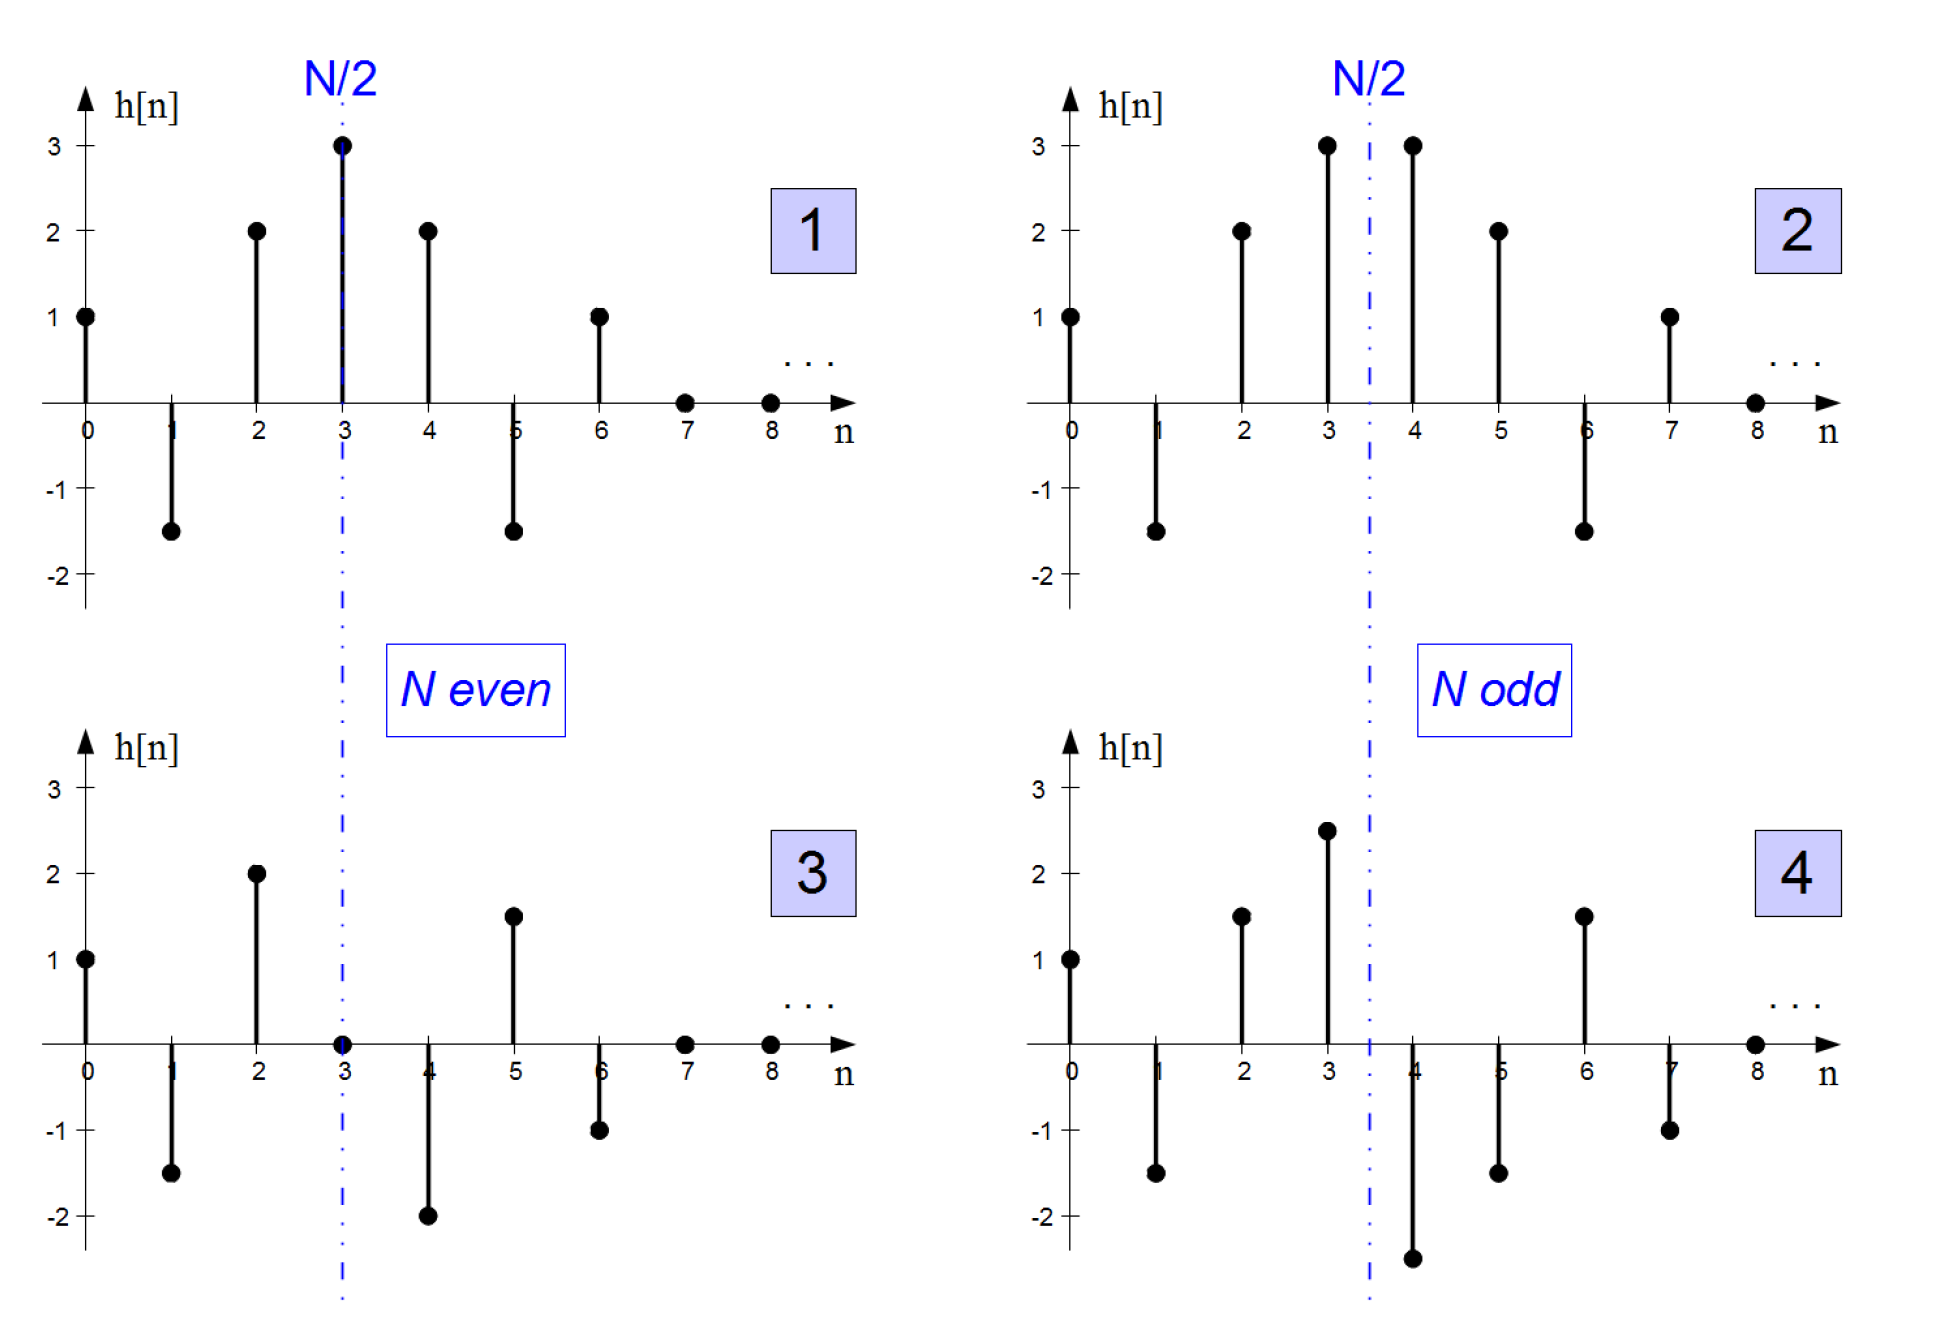
\includegraphics[width=.7\textwidth]{../fig/fir_filter}
	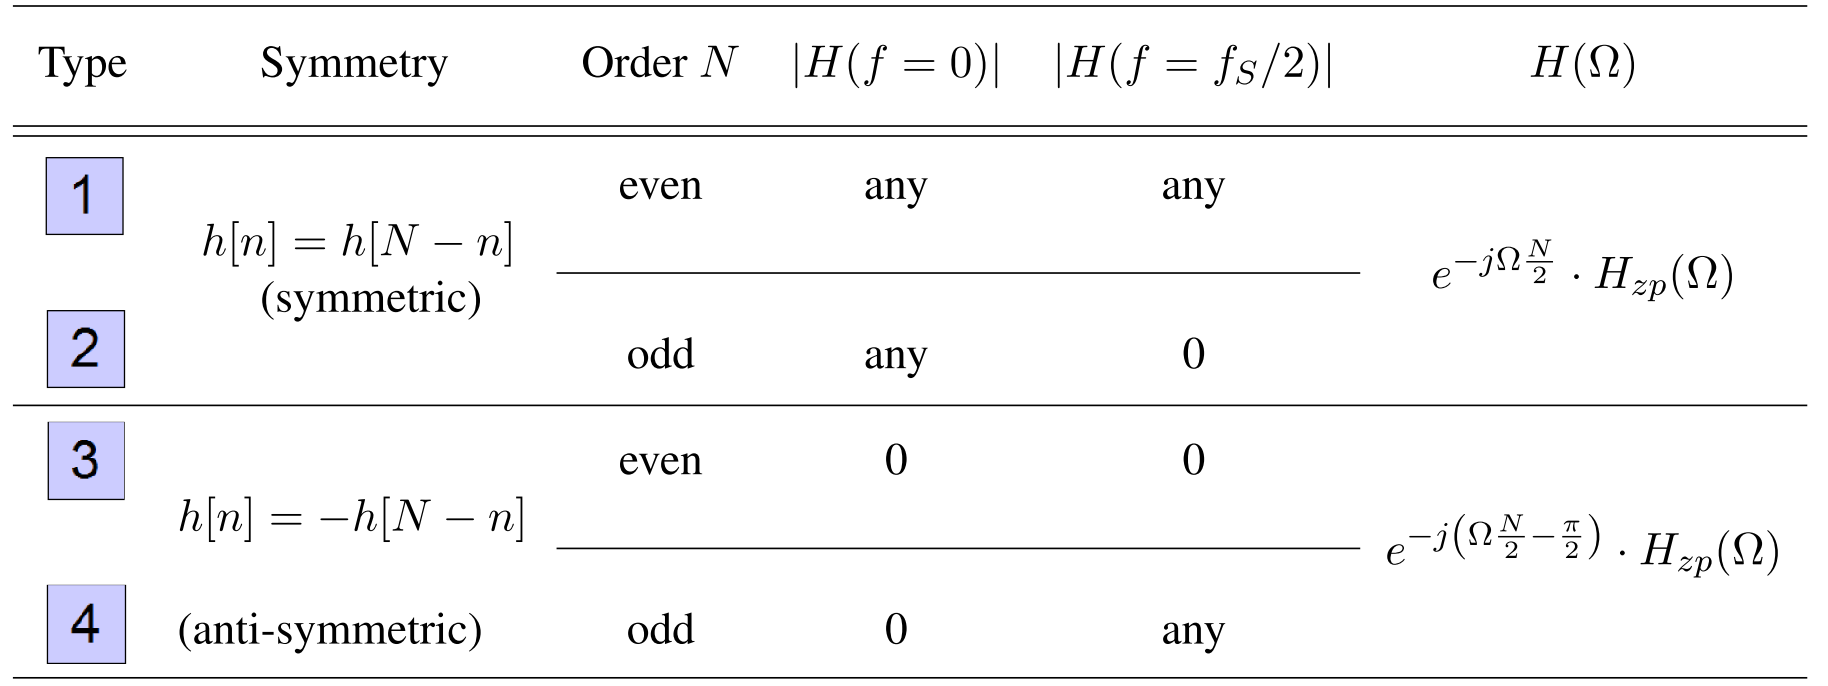
\includegraphics[width=.75\textwidth]{../fig/fir_table}
\end{center}
\textbf{Anmerkung Phasensprung \& Gegenmassnahme:\\}
Im Stop-Band symmetrischer FIR-Filter können 180\textdegree -Phasensprünge auftreten.
Sie entstehen bei jedem Frequenzpunkt von komplex-konjugierten Nullstellen am Einheitskreis.
Im Normalfall werden sie toleriert, da die Dämpfung im Stopp-Band entscheidend ist. 
Ansonsten können die Sprünge durch Duplikate der komplex-konjugierten Nullstellen-Paare 
eliminiert werden. Achtung: Dies erhöht jedoch die Gruppenlaufzeit durch die entstehende
höhere Ordnung.\\\\
\textbf{Anmerkung Gruppenlaufzeit:\\} 
Symmetrische FIR-Filter weisen eine lineare Gruppenlaufzeit auf mit $N/2$ Samples.
Die Nullstellen dieser Filter treten in reziproken Paaren auf (z.B. bei $-1/2$ und $-2$).
%===============================================================================
\subsection{Window Design Methode}
Der Matlab-Befehl \verb|fir1()| verwendet die Window Design Methode. Es wird mit 
der Impulsantwort eines idealen Tiefpass-Filters mit Cutoff-Frequency $f_c$ gestartet. 
Die ideale Impulsantwort ist nicht endlich. Sie wird auf eine endliche Länge von $N+1$ 
begrenzt und um $N/2$ Samples geshiftet. 
\[ h_{d_{TP}}[n]= \frac{sin(\Omega_c \cdot n)}{n \cdot \pi} \qquad \qquad
			\Omega_c = 2 \cdot \pi \cdot \frac{f_c}{f_S}, \text{ }n = \bigg\{\frac{-N}{2},...,\frac{N}{2} \bigg\} \]
Für den Wert von $h_{d_{TP}}[0]$ muss aufgrund der Nulldivision die Regeln von L'Hospital angewendet werden (normalisiert auf $f_S$!):
\[ 
	\frac{\text{d}}{\text{d}n}  \left( \frac{ sin(2\cdot f_c \cdot \pi \cdot n} {\pi \cdot n} \right)\bigg|_{n=0}= 
	\frac{2\cdot f_c \cdot \pi \cdot cos(2\cdot f_c \cdot \pi \cdot 0)}{\pi} = 2 \cdot f_c \qquad \qquad h_{d_{TP}}[0]= \frac{2 \cdot f_c}{f_S}
\]
\begin{enumerate}[noitemsep,topsep=3pt]
	\item Ideale Tiefpass Übertragungsfunktion
	\item Ideale Impulsantwort (nicht endlich)
	\item Begrenzen der Impulsantwort mittels Fenster
	\item Geshiftete Impulsantwort zur praktischen Umsetzung
\end{enumerate}
\begin{center}
	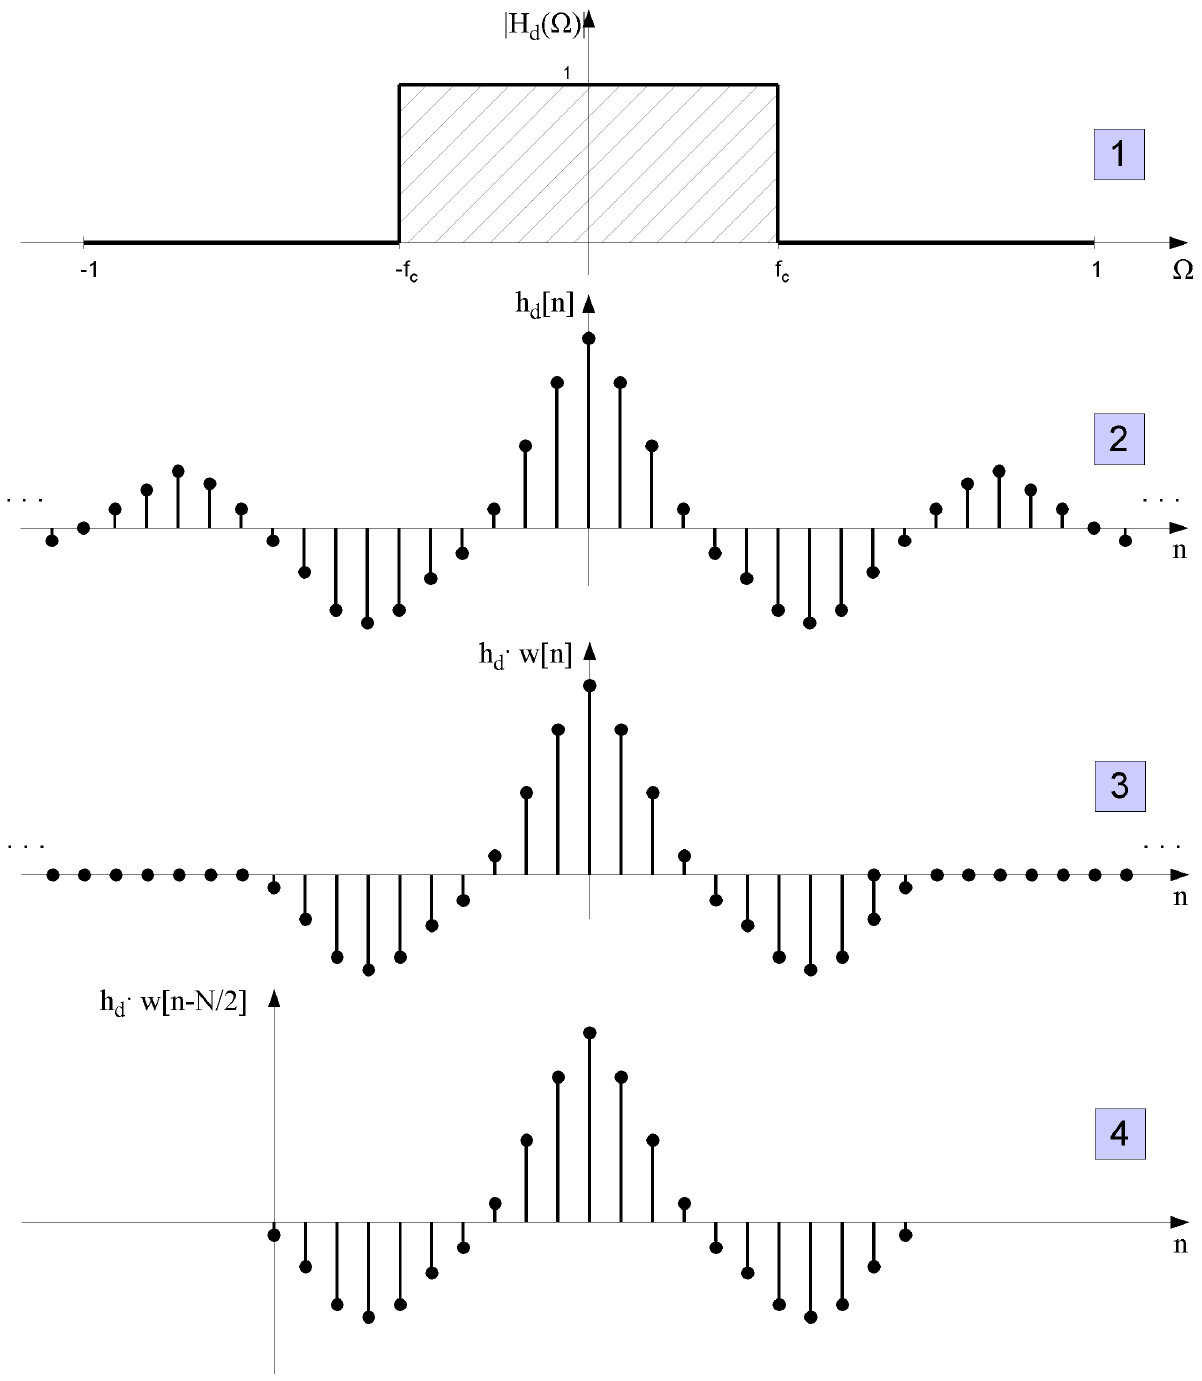
\includegraphics[width=.625\textwidth]{../fig/window_design_methode}
\end{center}
\textbf{Vorgehen für Band- und Hochpass:\\}
Band- und Hochpass-Filter werden durch die Summe oder Differenz von Tiefpass-Filtern
mit unterschiedlichen Cutoff-Frequencies bestimmt. Beispiel von Hochpass: Tiefpass mit 
$f_c = f_S/2$ minus ein anderer Tiefpass mit der $f_c$. Die Impulsantwort des 
Hochpassfilters lautet demnach:
\begin{align*}
	h_{d_{HP}}[n]&= \frac{sin(n \cdot \pi)}{n \cdot \pi} - \frac{sin(\Omega_c \cdot n)}{n \cdot \pi} 
	= -h_{d_{TP}}[n], \text{ wobei: } h_{d_{HP}}[0]= 1 - h_{d_{TP}}[0]  \\
	&=\{ ...,\ -h_{d_{TP}}[-2],\ -h_{d_{TP}}[-1],\ 1-h_{d_{TP}}[0],\ -h_{d_{TP}}[1],\ -h_{d_{TP}}[2],\ ... \} 
\end{align*}
\textbf{Zusammenhang zwischen Overshoot, Übergangsband, Ordnung \& Window-Typ:\\}
Das Anwenden des Windows entspricht einer Faltung des idealen Frequenzgangs mit
einem Rechteckfenster. Dadurch entsteht ein Overshoot bei den Übergängen der Bänder. 
Der Overshoot kann durch erhöhen von $N$ nicht reduziert werden, jedoch wird dadurch 
die Breite des Übergangsbereichs verringert. Um den Overshoot zu verringern, muss 
ein anderes Windows als das Rechteck eingesetzt werden. Das Übergangsband wird dadurch
jedoch etwas breiter.
%===============================================================================
\subsection{Alternative Designmethoden}
\textbf{Equiripple:} Erzielt teils tiefere Filter-Ordnung $N$ für dieselben Spezifikationen,
da der Rippel im Durchlass- und Stoppband gewichtet werden kann. Der Filter weisst dabei  
eine konstante Rippel-Amplitude auf.\\
\textbf{Frequenz-Sampling:} Man sampelt den idealen Frequenzgang $H_d(\Omega)$ an $N$ 
Sample-Punkten in identisch grossem Abstand. Durch Anwenden der IDFT zwischen 0 ... $2\pi$
erhält man die Impulsantwort.
%===============================================================================
\subsection{FIR-Kammfilter}
z-Übertragungsfunktion des Kammfilters $N$-ter Ordnung:
\[ H(z)\ =\ 1\ \pm z^{-N} \]
Impulsantwort:
\[ h[k]= [b_0 \ 0 \dots 0 \ b_N] =  [1 \ 0 \dots 0 \ \pm1] \]
Alle $N$ Pole sind im Ursprung. Die Nullstellen ergeben sich aus den Einheitswurzeln, 
bei $b_N=1$ haben diese noch eine Phasenverschiebung (siehe linker Fall unten).
\begin{center}
	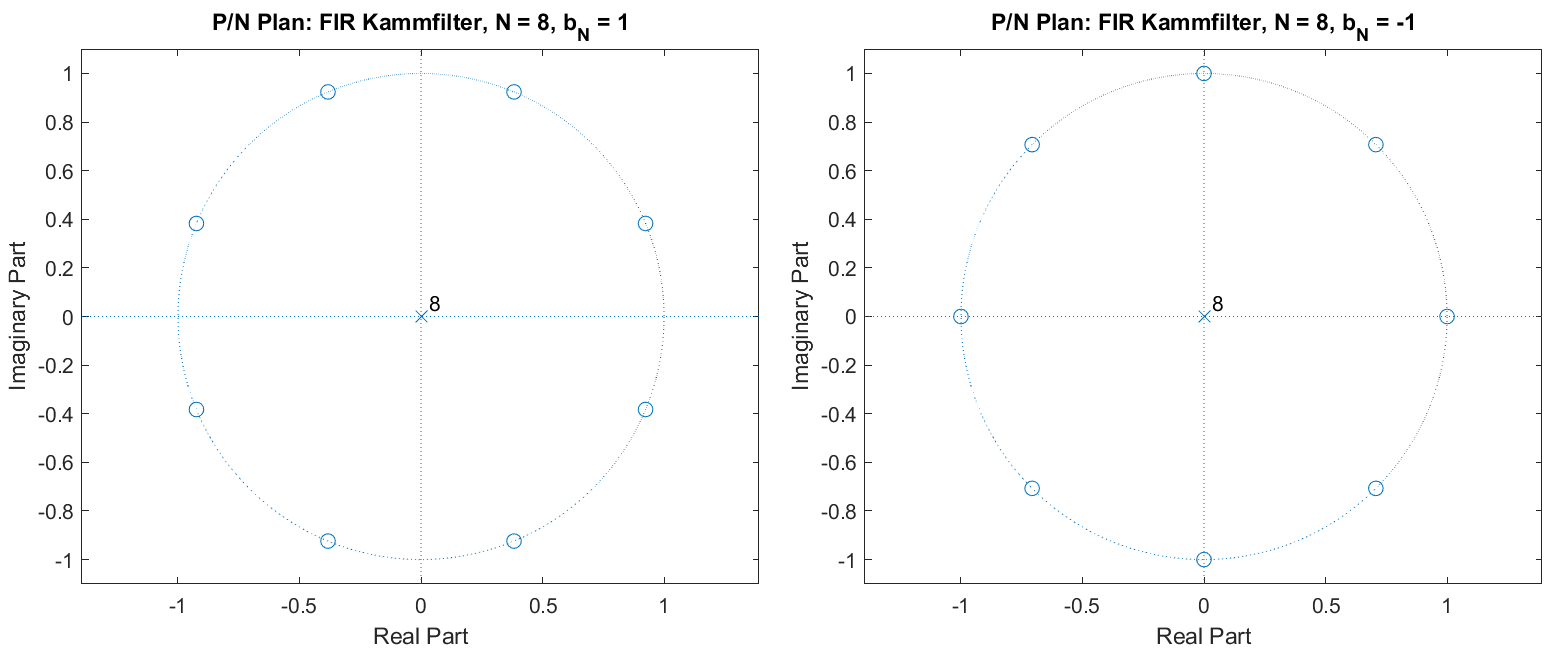
\includegraphics[width=0.875\textwidth]{../fig/fir_comb}
\end{center}\vspace{-4mm}
%===============================================================================
\subsection{Kanalausgleich mittels FIR}
Angenommen, ein Kanal verzerrt das Signal durch Echos. Die Impulsantwort ist endlich. 
Mittels Channel Equalization kann der Kanal entzerrt werden. Dazu eignet sich folgendes
Vorgehen, um die Koeffizienten des Filters in Echtzeit zu berechnen. Der Aufwand bezieht 
sich auf die Anzahl realer Multiplikationen (1 cpl Mul = 2 real Mul): 
\begin{enumerate}[noitemsep,topsep=3pt]
	\item FFT der Impulsantwort (Aufwand: $\left[\frac{N}{2}\cdot\log_2N\right]$)
	\item Invertierung aller Spektralwerte (Aufwand: $\left[N\right]$)
	\item IFFT des invertierten Spektrums (Aufwand: $\left[\frac{N}{2}\cdot\log_2N\right]$)
\end{enumerate}
Totaler Aufwand an realwertigen Multiplikationen: $2N + 2N\log_2N$
\newpage

%===============================================================================
\section{IIR-Filter}
\subsection{Eigenschaften}
Bei IIR-Filtern ist die Ordnung des Nenners $M>0$, es existieren also Polstellen bei 
$z\neq0$. Die Impulsantwort dieser Filter ist theoretisch unendlich. Generell kann mit 
einem IIR-Filter mit tieferer Ordnung derselbe Amplitudengang wie mit einem FIR-Filter 
erreicht werden. Die Laufzeit verkürzt sich dadurch, eine konstante Gruppenlaufzeit 
lässt sich jedoch nicht realisieren. Durch Quantisierungsfehler können IIR-Filter instabil 
werden. Tabellarischer Vergleich:
\begin{center}
	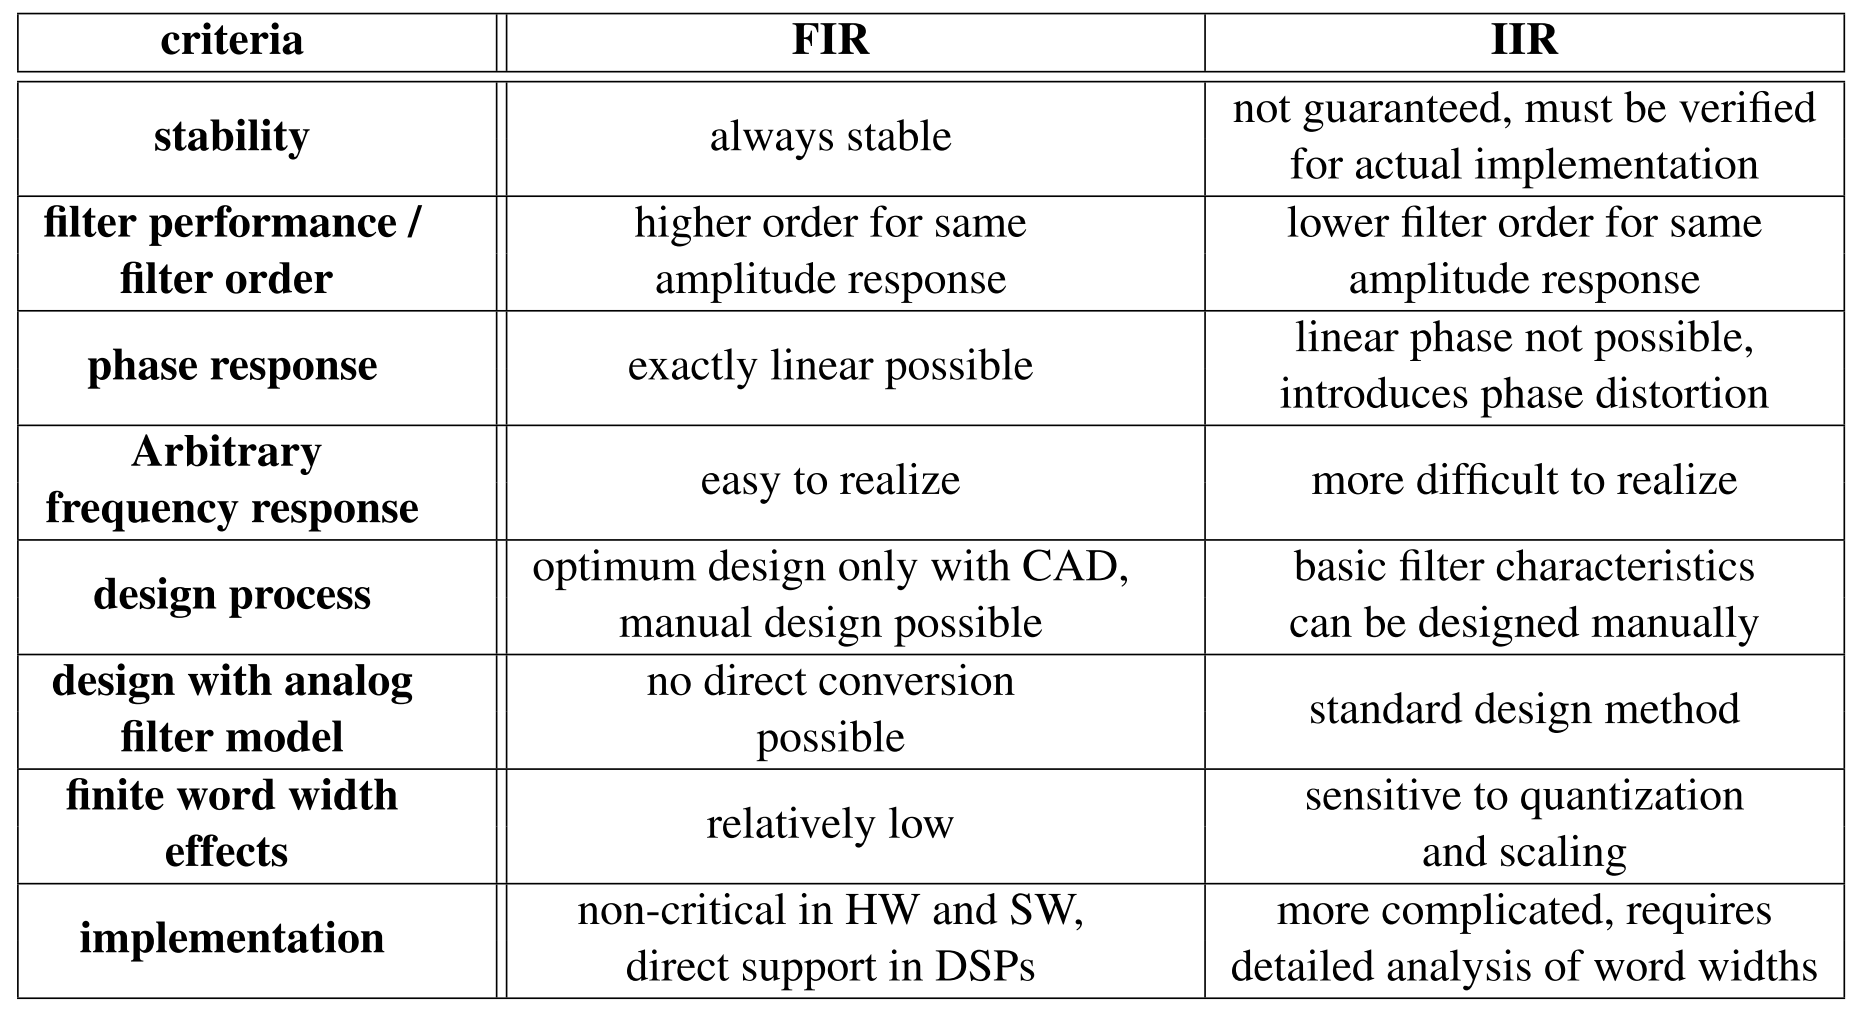
\includegraphics[width=.8\textwidth]{../fig/fir_vs_iir}
\end{center}
%===============================================================================
\subsection{IIR-Design mittels Impulsinvarianz-Transformation (Tiefpass)}
Die Impulsantwort des digitalen IIR-Filters wird durch Sampling der Impulsantwort des
analogen Prototyp-Filters ermittelt. Um Aliasing zu verhindern, muss $f_S$ mindestens doppelt so gross wie die höchste 
Durchlass-Frequenz des analogen Prototypen-Filters sein. Die Methode ist demnach nur 
für Tiefpass, jedoch nicht für andere Filter geeignet.
\[ h[n] = h_a(n \cdot T_S) \qquad n=0,1,2,... \]
Umformung von der $p$-Ebene zur $z$-Ebene:
\[ z = \e^{pT_S} \]
\begin{center}
	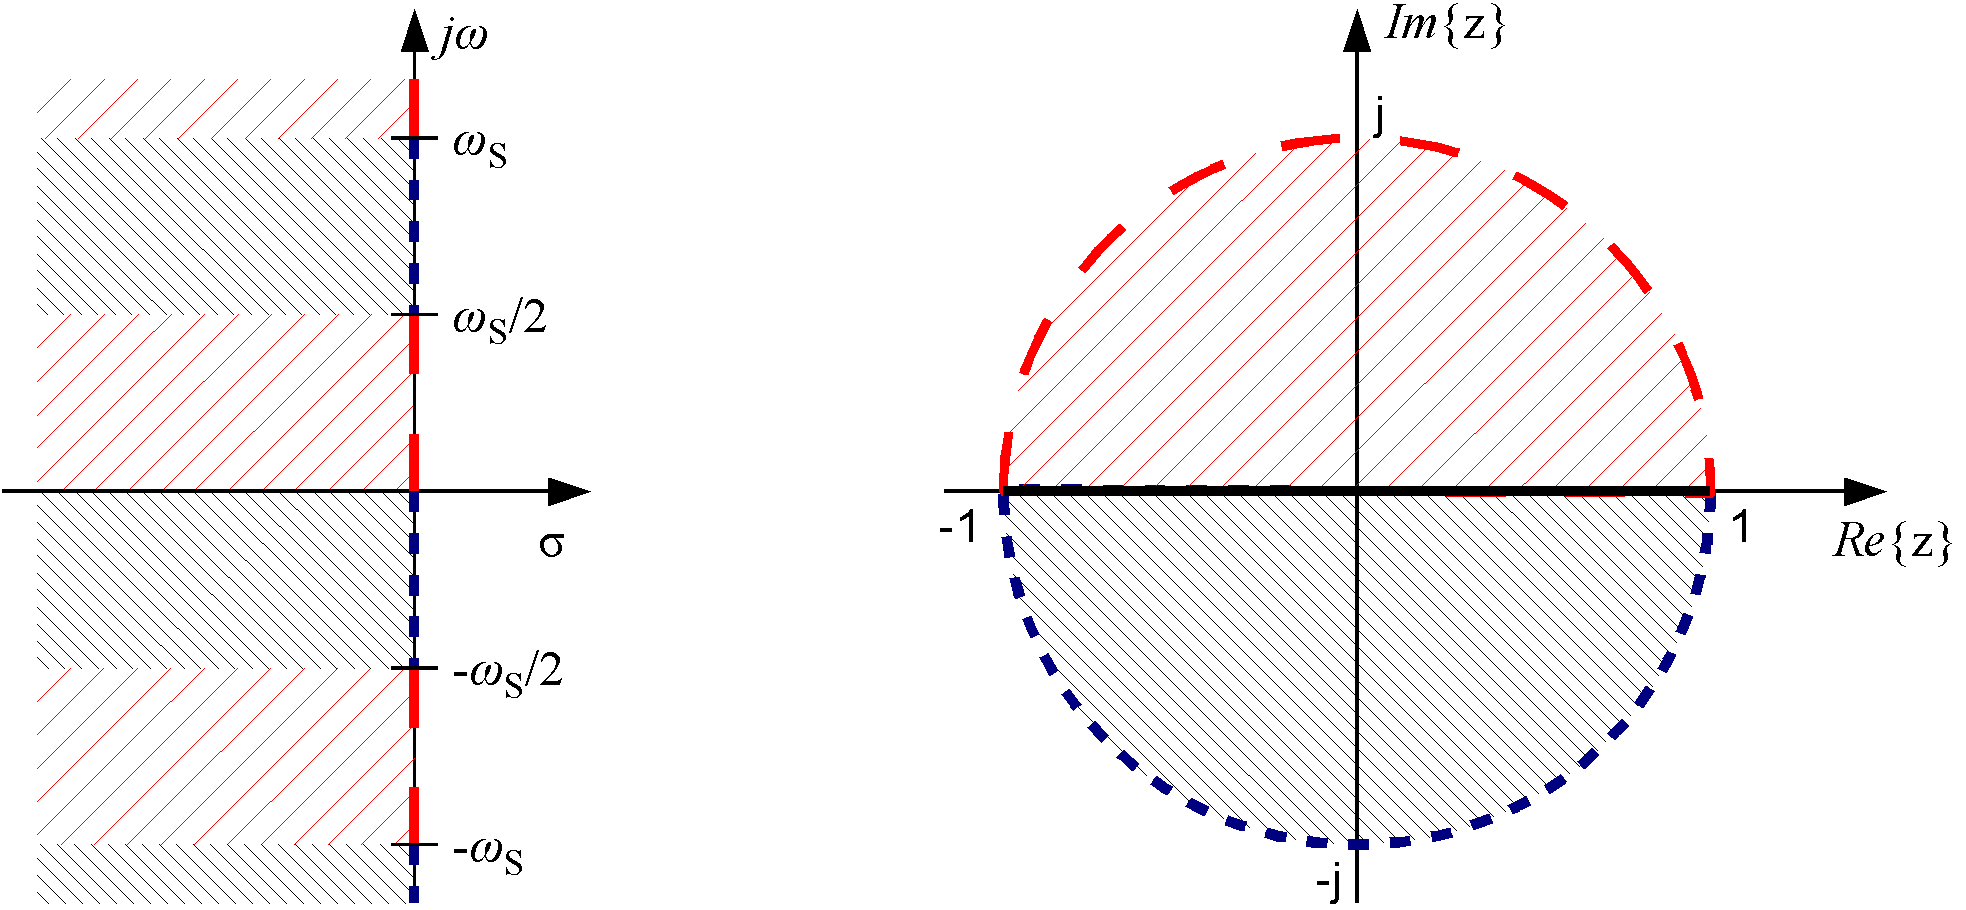
\includegraphics[width=.7\textwidth]{../fig/mapping_p_to_z_plane}
\end{center}
\newpage

%===============================================================================
\section{Implementationsaspekte}
Die Wahl der Sampling-Frequenz muss gut durchdacht sein. Bei zu hoher Sampling Frequenz entstehen Probleme:
\begin{itemize}[noitemsep,topsep=3pt]
	\item Grösserer Rechenaufwand, da mehr Samples in vorgegebener Zeit bearbeitet werden müssen.
	\item Je kleiner der Frequenzabstand zwischen Pass- und Stoppband wird, desto steiler wird die Filterkurve. 
	Dies wiederum erzwingt eine höhere Ordnung, was erneut den Rechenaufwand erhöht.
	\item Je näher Pol- und Nullstellen der Transferfunktion in der $z$-Ebene kommen, desto höher die Sensitivität 
	gegenüber Quantisierungseffekten der Koeffizienten. 
\end{itemize}
%===============================================================================
\subsection{Implementation von IIR-Filtern}
Der IIR-Filter kann als eine Kette von "'biquads"' implementiert werden. Dabei wird die
Übertragungsfunktion in $L$ Bläcke aufgeteilt, welche jeweils einen konjugiert-
komplexen Pol haben:
\[ H(z) = K \cdot \frac{(z-z_1)(z-z_1^*)}{(z-p_1)(z-p_1^*)}\cdot\ldots\cdot
	\frac{(z-z_L)(z-z_L^*)}{(z-p_L)(z-p_L^*)} \]
Die Sub-Übertragungsfunktionen werden dabei in der "'Direct Form I"' oder in der "'Transposed 
Direct Form I"' implementiert. Beispiel mit biquads zweiter Ordnung in der "'Transposed Direct 
Form II"':
\begin{center}
	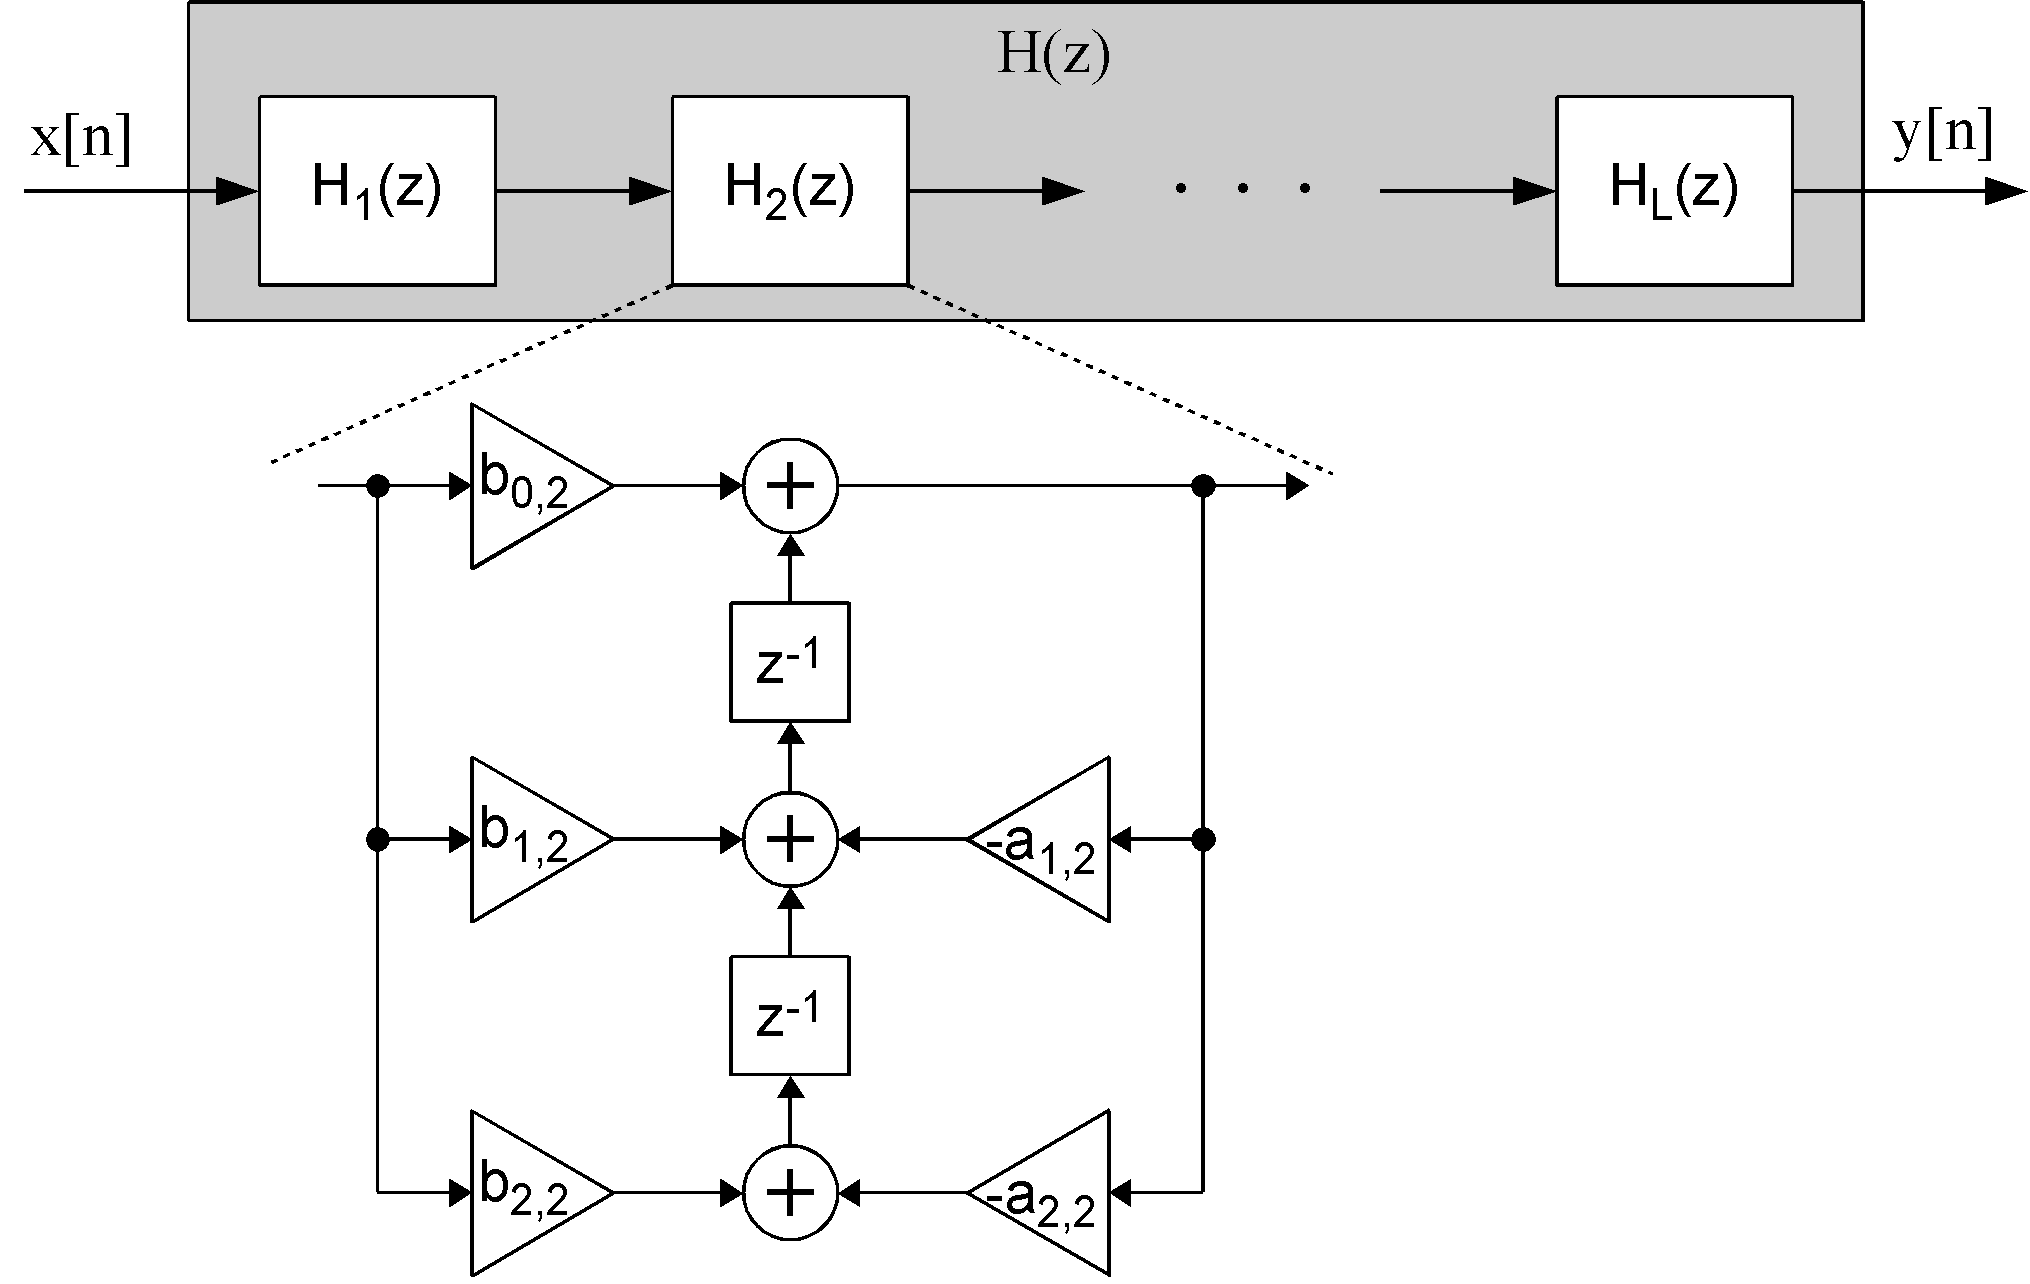
\includegraphics[width=.65\textwidth]{../fig/iir_implementation_biquads}
\end{center}
Matlab-Befehl zur Umwandlung der Koeffizienten von $H(z)$ in die Koeffizienten von $H_1(z), ..., H_L(z)$: \verb|tf2sos()|
\subsection{Fixkomma-Implementation}
Die Implementation im Fixkomma-Format ist resourceneffizienter als das Fliesskomma-Format.
Bei einer Fix-Point Implementierung mit $W$ Bits ($b_k$) und $F$ Nachkommastellen ist
der dezimale Wert:
\[ D_{ufix} = \sum_{k=0}^{W-1}b_k \cdot 2^{k-F} \]
Für Zahlen im Zweierkomplement ergibt sich der dezimale Wert wie folgt:
\[ D_{sfix} = -b_{W-1} \cdot 2^{W-F-1} + \sum_{k=0}^{W-2} b_k \cdot 2^{k-F} \]
\textbf{Overflow:}
Kann durch Hinzufügen zusätzlicher MSBs, einer Sättigung (Begrenzen der Zahlen auf grösste 
repräsentierbare Zahl) oder "'wrap-around"' (zählt beim kleinsten Wert weiter) erreicht werden.\\\\ 
\textbf{Underflow:}
Das Resultat kann aufgrund fehlender LSBs (Auflösung) nicht angezeigt werden. Zu den 
Massnahmen zählen Abschneiden (LSBs vernachlässigen) oder Runden (auf die nächst gelegene repräsentierbare Zahl).